%%%%%%%%%%%%%%%%%%%%%%%%%%%%%%%%%%%%%%%%%
% Visualization and Visual Data Analysis
%
% Author:
% Benjamin Neckam
% Alexander Gelb
%
%%%%%%%%%%%%%%%%%%%%%%%%%%%%%%%%%%%%%%%%%

\documentclass{article}

\usepackage[utf8]{inputenc}
\usepackage{textcomp}
\usepackage{graphicx}
\usepackage{url}

\begin{document}
\title{Visualization and Visual Data Analysis}
\author{Gelb, Alexander; Neckam, Benjamin}
\maketitle
\section{M2 - Lo-Fi Prototyping}
\subsection{Proposed visualization solution}
The user interface is oriented on programs like "Tableau" or "Glue" because we think it is the most easiest and most intuitive way to work with data. Figure 1 shows a very rough prototype of it with just two main parts:\\
\begin{itemize}
\item Information view
\item Plot view
\end{itemize}
\subsubsection{Information view}
At the moment the information view, figure 2, is divided in two parts, "Data" and "Options". Data provides some information about the dataset itself like name of the table, number of columns, rows and entries or column names. Options should give the possibility to add plots, interactions and other things to the plot view.
\subsubsection{Plot view}
The plot view is the area where, like the name tells us, all the plots appear and the interaction happens.
\subsubsection{Graph proposals}
Since we did not get a real specification of the customer what he would like to get visualize and just told us to try out whatever we want, we came up with a few ideas which might be interesting for astronomers. Unfortunately there are just 4 things, distance to sun, color, position and amount of stars which can be plotted in a meaningful manner, which made it really hard to find good plotting examples. At least we got six ideas so far and hope that the process of working with the data more intense we get new ideas for new plots.
\begin{itemize}
\item Scatterplot which shows the number of stars compared to the distance of the sun. (figure 3)\\
\\
Advantage is to get a good overview of how the stars are distributed in the area around the sun.
An disadvantage will be the confusion if there are to many stars and therefore no chance to find any patterns or other interesting things.
\item 3D representation of star clusters around the sun. (figure 4)\\
\\
Since the universe is a three dimensional space it is easier to see where specific star clusters are located but we are not sure if it is possible to create such a visualization with D3.
\item The ratio of hot and cold stars. (figure 5)\\
\\
It is very easy to understand but it can give a wrong picture of the data.
\item Bar chart showing the size of specific star clusters. (figure 6)\\
\\
Like the pie it is very self explaining but if for example the scale of the y-axis is chosen wrong at can lead to false interpretation.
\item Line graph showing how the velocity behaves to the distance to the sun. (figure 7)\\
\\
An advantage of this view is that it shows in a good way of how the velocity changes with the distance to the sun but like with the bar chart choosing a good scale for the axis is important.
\item Shows the movement of a star in a certain time. (figure 8)\\
\\

\end{itemize}
\subsubsection{Interactions}
One dashboard could be to combine figure 4, 5 and 6. While figure 4 shows the star clusters around the sun in three dimensional context, figure 5 can give us an overview how the ratio of hot and cold stars in the data are. To see how many stars are inside of a cluster, figure 5 can provide the information with a bar chart. The interactions could be to click on a specific cluster in the three dimensional representation and figure 5 and 6 updates their values corresponding to the selected cluster. An other interaction is when you just want to see all the hot stars you can select them in figure 5 and all other plots updates their view to show only the hot ones.\\
\\
The second idea is to combine figure 4 and 7. If a cluster is selected figure 7 shows the distance of the nearest star of the cluster to the sun to the farthest and how the velocity of the selected stars behaves concerning the distance to the sun.\\
\\
The third interaction can happen between figure 3, 7 and 8. If selecting a single star from figure 3, we can see how it moves over period of time and how the velocity changed with the distance to the sun.

\begin{figure}[!h]
\centering
    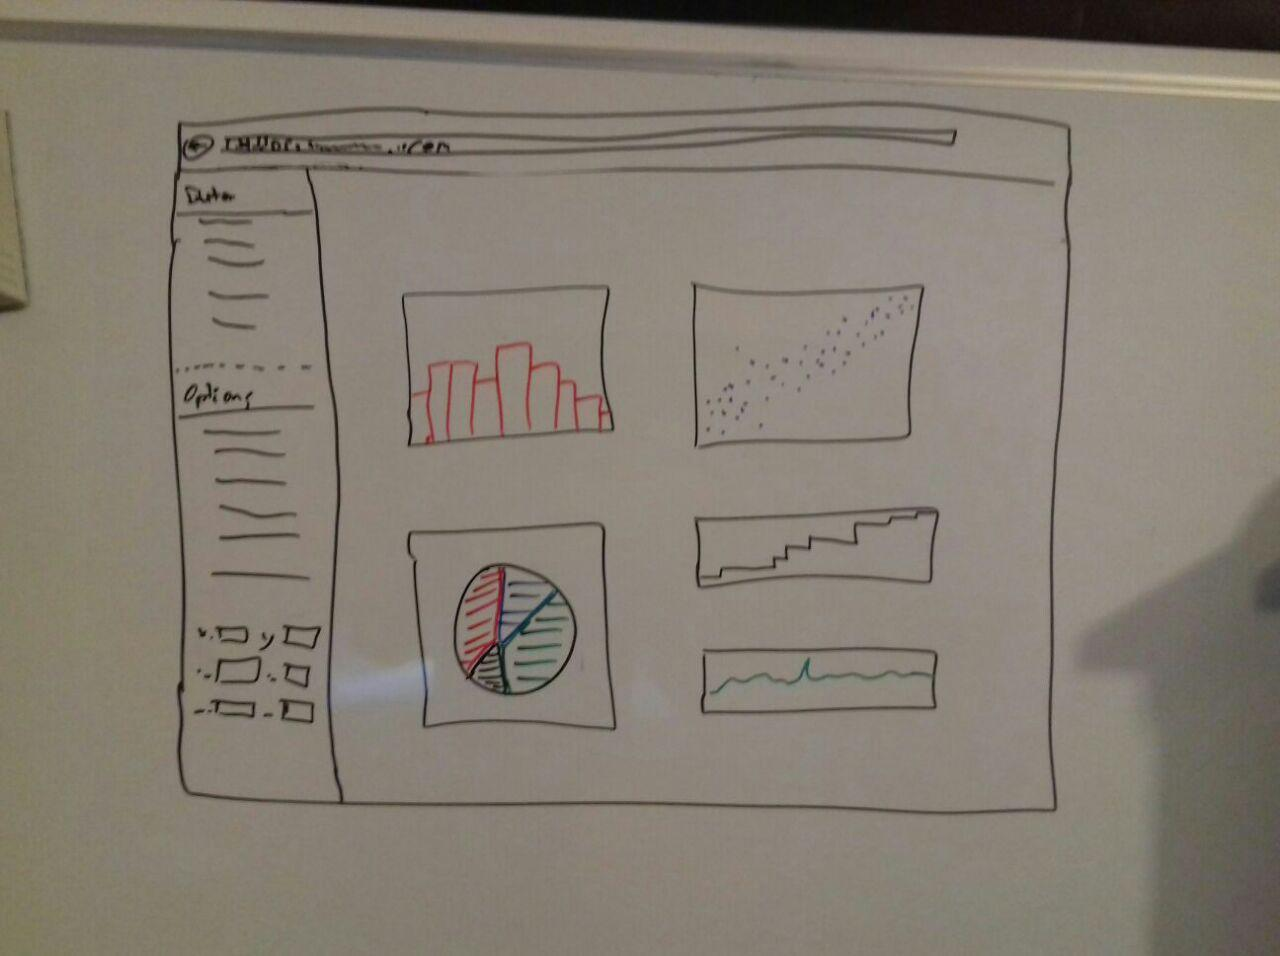
\includegraphics[width=\textwidth]{Prototype1.jpg}
	\caption{User interface}
	\label{fig1}
\end{figure}
\begin{figure}
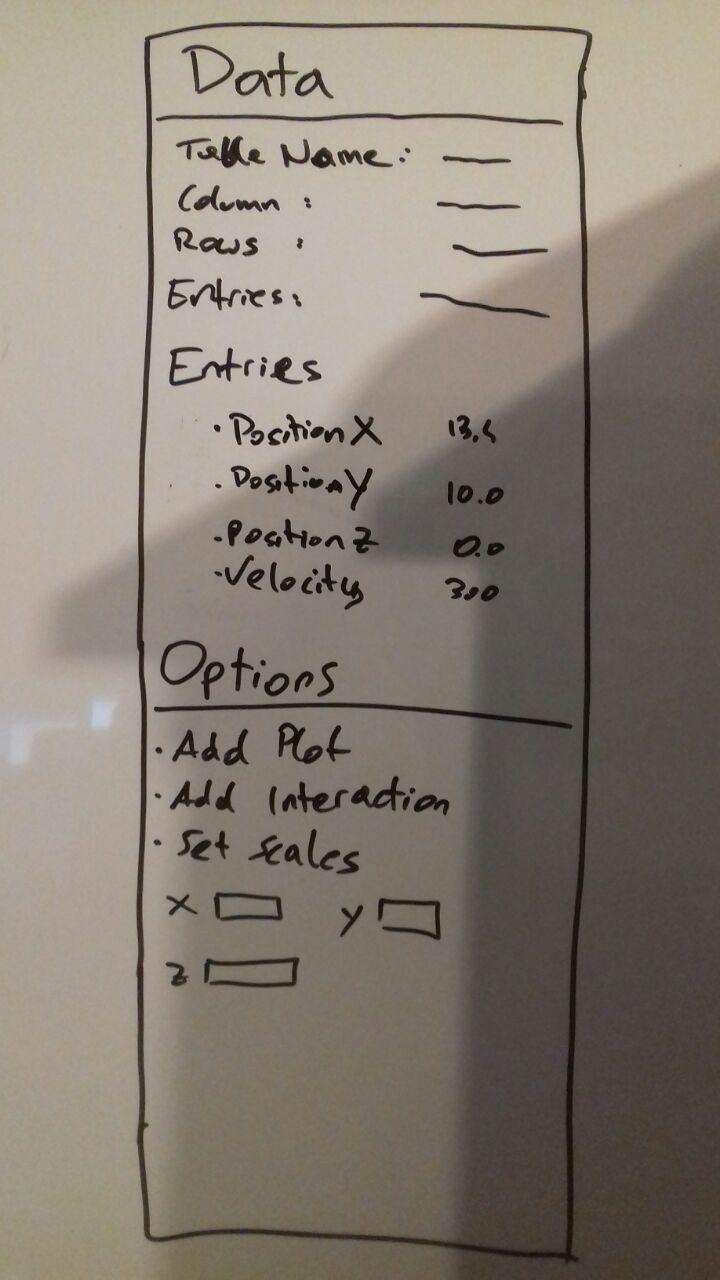
\includegraphics[width=\textwidth]{InformationView.jpg}
	\caption{Information view}
	\label{fig2}
\end{figure}
\begin{figure}
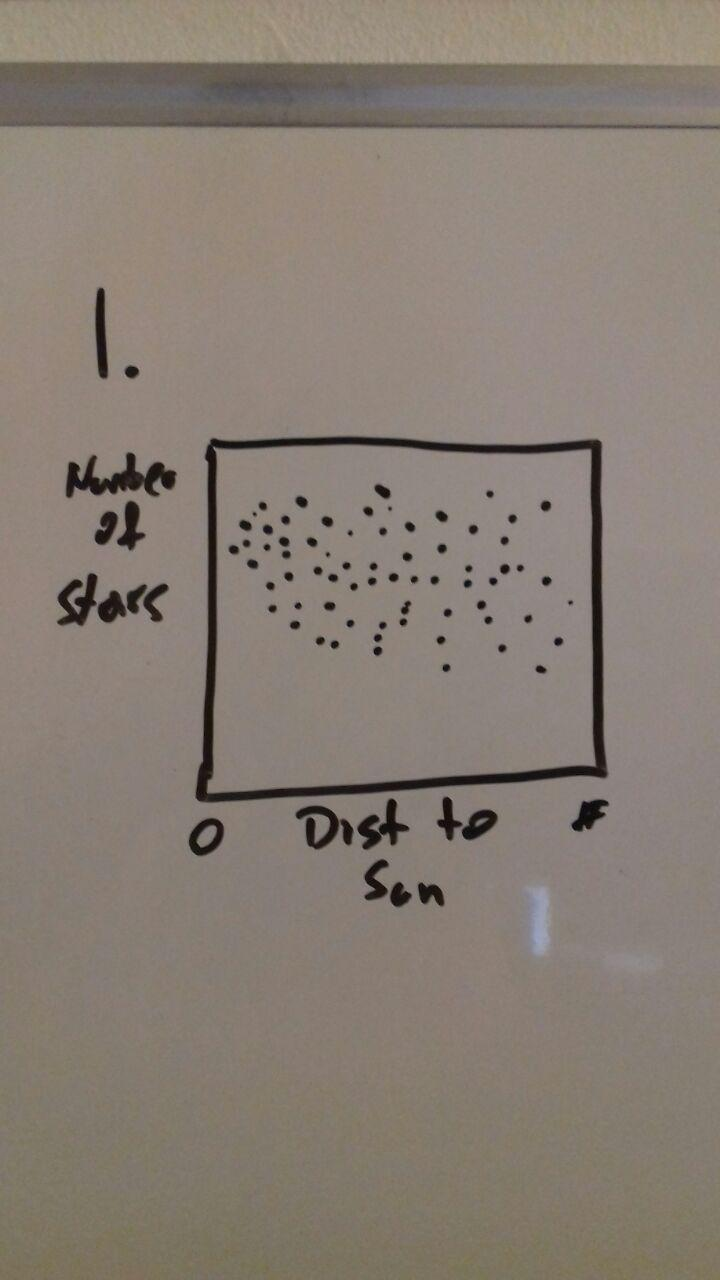
\includegraphics[width=\textwidth]{NumbStarsDistSun.jpg}
	\caption{Scatterplot}
	\label{fig3}
\end{figure}
\begin{figure}
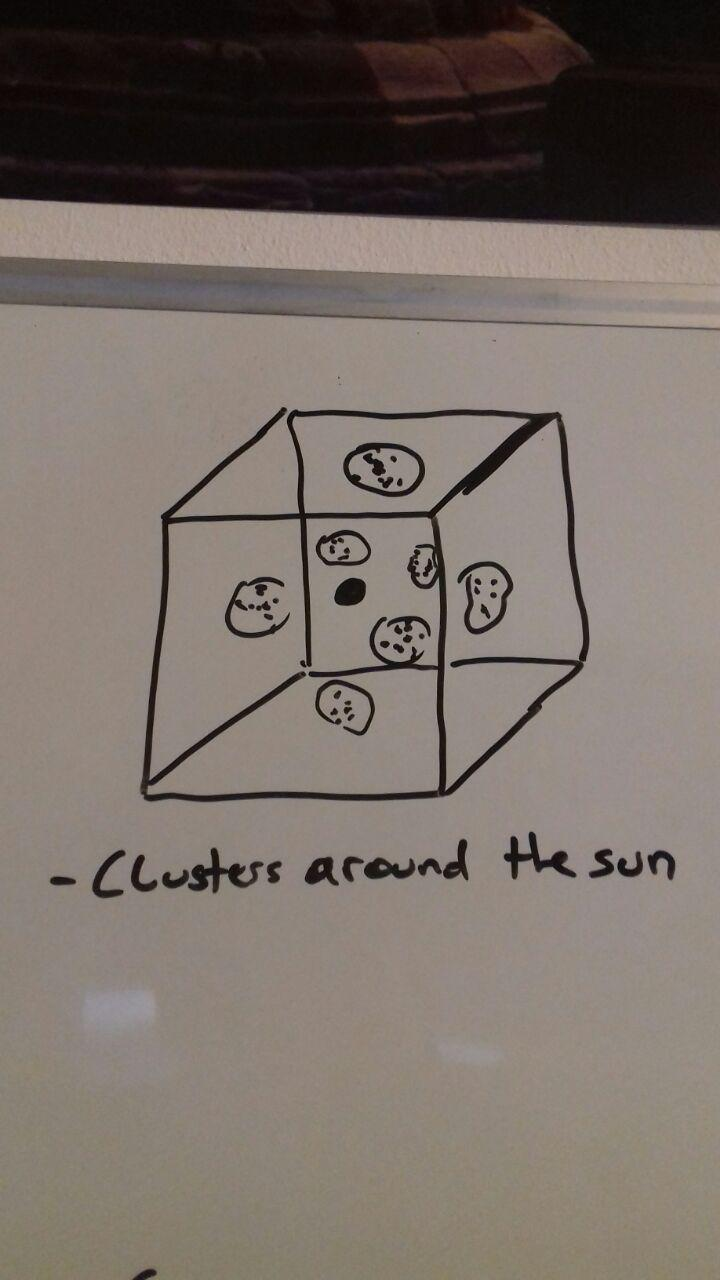
\includegraphics[width=\textwidth]{ClustersSun3d.jpg}
	\caption{3D visualization}
	\label{fig4}
\end{figure}
\begin{figure}
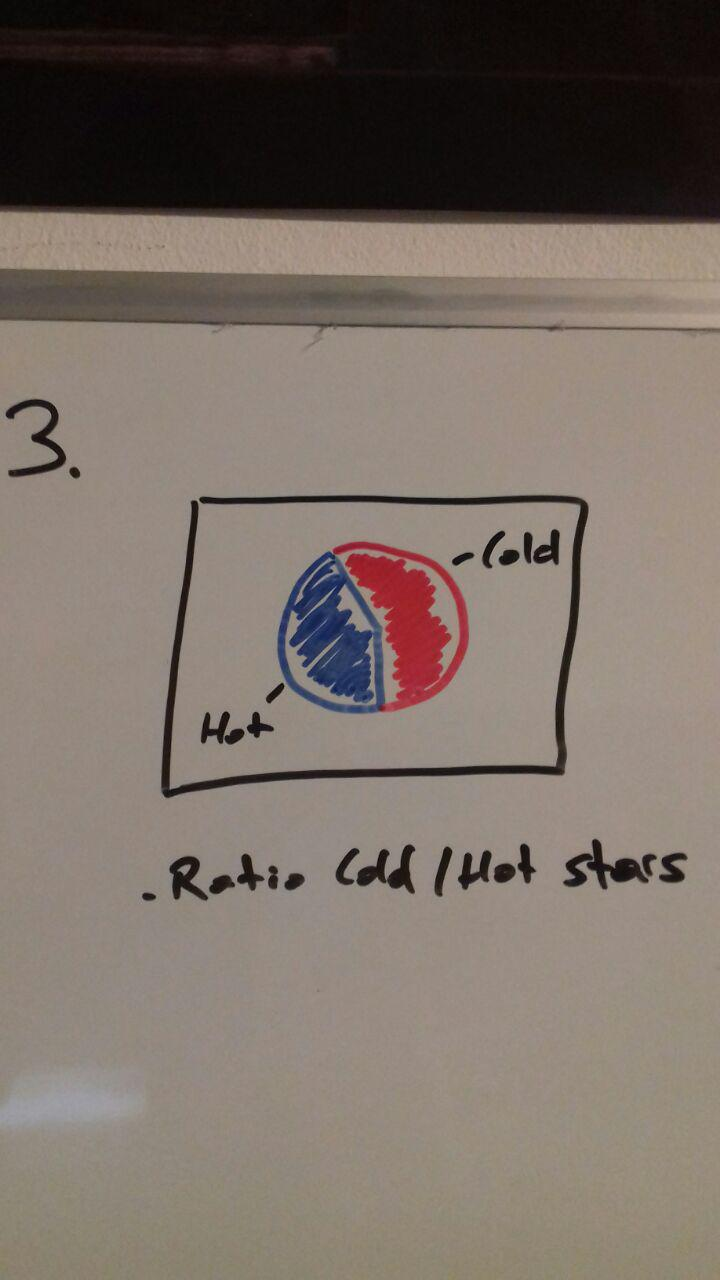
\includegraphics[width=\textwidth]{HotColdRatio.jpg}
	\caption{Pie chart}
	\label{fig5}
\end{figure}
\begin{figure}
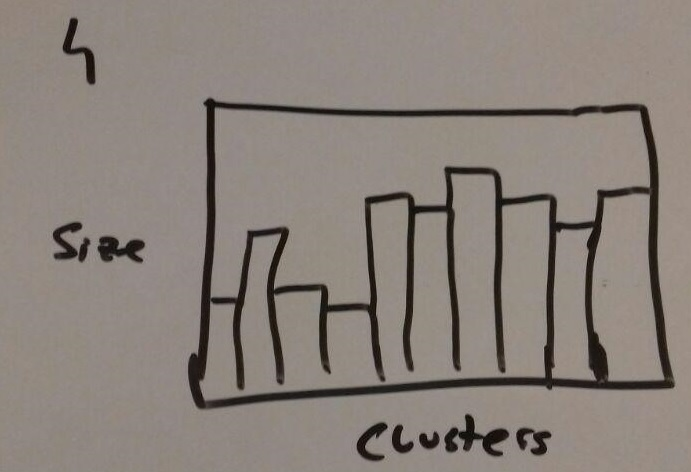
\includegraphics[width=\textwidth]{SizeClusters.jpg}
	\caption{Bar diagram}
	\label{fig6}
\end{figure}
\begin{figure}
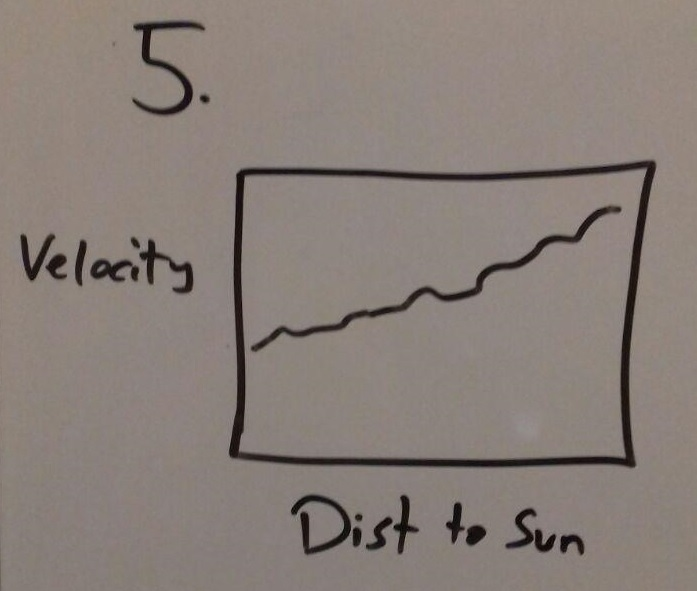
\includegraphics[width=\textwidth]{VelocityDist.jpg}
	\caption{Line graph}
	\label{fig7}
\end{figure}
\begin{figure}
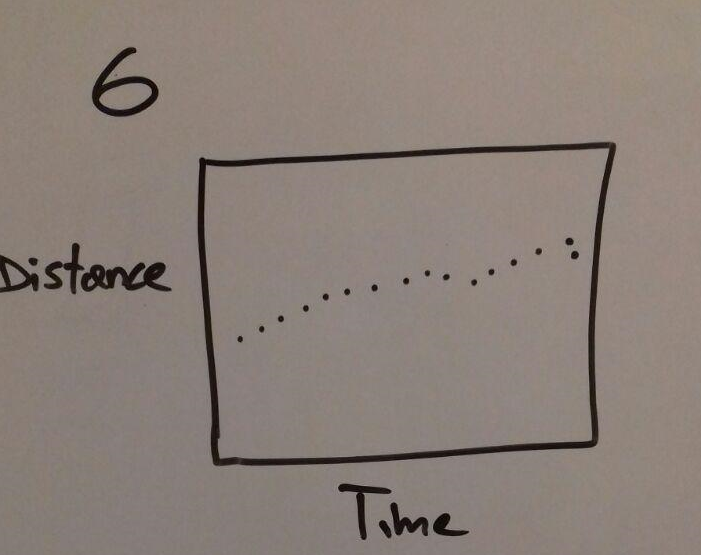
\includegraphics[width=\textwidth]{DistanceTime.jpg}
	\caption{Dot plot}
	\label{fig8}
\end{figure}
\end{document}